%\documentclass[10pt,preprint]{aastex}
\documentclass[apj]{emulateapj}
\usepackage{txfonts}
\usepackage{graphicx}
\usepackage{natbib}

\newcommand{\kms}{${\rm km \; s^{-1}}$}

\shorttitle{Local Number Density Environments of Massive Galaxies}
\shortauthors{Lifset}

\begin{document} 
\title{Local Number Density Environments of Massive Galaxies}

\author{Noah Lifset\altaffilmark{1}, 3D-HST}
\altaffiltext{1}{Yale University, 260 Whitney Ave., New Haven, CT 06511}

\begin{abstract}

We study the local galaxy number density environments of very massive galaxies in the 3d-hst survey. We select galaxies with mass greater than 10 \textsuperscript{11} solar masses and with a redshift between 0.5 and 2.5. Using both the nth nearest and counts in aperture radius calculations for local galaxy number density, we are able to study both the immediate environment and general environment. sorting the galaxies into  redshift and mass bins, we study the relationship between local galaxy number density, redshift, and mass. We find an increased number density in the local environment for the most massive galaxies of our sample. We also find that there is an inverse correlation with galaxy number density and redshift. This paper is largely an extension of Tal (2013)~\cite{2013ApJ...769...31T}.

\end{abstract}
\keywords{}

\section{Introduction}

The properties of galaxies are largely affected by their local environments and vice-versa. Local galaxy number density has been shown to correlate with a number of important properties, such as morphology, mass, star formation rate, and stellar colors (link to articles that Tomer links to in his nitroduction?). Less is known about local galaxy number density and redshift, especially at Z\textgreater1. Tomer Tal has studied this relationship up to a redshift of 1.6 Tal (2013)~\cite{2013ApJ...769...31T}. Using a counts per aperture radius method with background subtraction, he found that redshift stayed largely constant, as well as mass.

Here, we use a similar method for galaxy number density, as well as the nth nearest method, to extend Tal's work to higher redshifts using the 3d-hst survey.

For this paper we adopt the following cosmological parameters: $\Omega_{m}$ = 0.3, $\Omega_{\Lambda}$ = 0.7, and \textit{H}$_{0}$ = 69.31 km (s Mpc)$^{-1}$.

\section{Sample Selection}

We use data from the galaxy survey 3d hst, which includes the fields Aegis, Cosmos, Goods-n, Goods-s, and uds. For our sample of massive galaxies to study, we made a few specifications. Galaxies are selected with a mass greater than 10 \textsuperscript{11} solar masses, although none exceed 10 \textsuperscript{11.8}. We also limit ourselves to galaxies within a redshift range of 0.5 to 2.5. In order to avoid errors in the calculation from selecting galaxies at the edge, and thus getting a less than expected number density, we do not select galaxies within 0.05 degrees of the edges of any field used.
We must also limit the selection of general galaxies used to calculate local number density. We only use galaxies within the same redshift range and with mass greater than 10 \textsuperscript{9,415} solar masses. The lower mass limit was taken from Tal (2014)~\cite{2014ApJ...789..164T}, and is used to keep completeness above 95\% at all redshifts.

\section{Data and Analysis}

We use two different methods for calculating local galaxy number density. The first, the nth nearest neighbor calculation, has been shown to be more accurate for immediate environments Cooper (2005)~\cite{2005ApJ...634..833C}. The second, counts in selected aperture radius, is more accurate for larger and more general environments Cooper (2005)~\cite{2005ApJ...634..833C}.

\subsection{Nth Nearest Calculation}

One of the most common ways of measuring local galaxy number density is using the distance to the nth nearest spectroscopically observed galaxy. Redshift information is used to restrict the pool of neighbors that can be selected from to a given velocity interval. This is done to avoid background and foreground sources. A redshift difference of 0.08 is used here to try and maintain completeness as best as possible. This cut off was selected based on suggestions by Cooper (2005)~\cite{2005ApJ...634..833C}, Tal (2012)~\cite{2012ApJ...751L...5T}, and Muldrew (2012)~\cite{2012MNRAS.419.2670M}. Thus the pool of galaxies that the nth nearest neighbor is being selected from is a cylinder, rather than a sphere. The nth nearest neighbor distance is expressed as a projected surface density $\Sigma$ $_{n}$. The calculation for the projected surface density is

 $$\Sigma_{n} = n / (\pi  R_{n}^{2})$$

 where R$_{n}$ is the distance to the nth nearest neighbor. 

It should be noted that there is no subraction of average background number density, unlike the counts in aperture radius method.



\subsection{Counts in Aperture Radius Calculation}

Another method for measuring local galaxy number density is counting the number of galaxies within a certain aperture radius. This method once again requires a redshift cut of 0.08. This was selected based on the relative photometric uncertainty between selected massive galaxies and general galaxies near them. The pool of galaxies counted is then also a cylinder rather than a sphere. The calculation for galaxy number density is simply
 $$\Sigma_{r} = n_{gal} / (\pi r^{2})$$
 where r is the selected aperture radius and n$_{gal}$ is the number of galaxies within that radius. Selecting many different aperture radii allows us to analyze the galaxy number density in both local and general environments. The larger aperture radii selected show the average number density within that entire radius, while smaller aperture radii are able to show the usually increased number density within a smaller radius.

In order to calculate the galaxy number density that is solely a result of the selected massive galaxies, an average background number density is subtracted after each normal $\Sigma_{r}$ calculation. In order to do this, for each selected massive galaxy, four different calculations are carried out for galaxy number density using the selected galaxy's field and redshift, but random coordinateswithin said field. These four calculations are then averaged and we have our averaged background number density. Subtracting this from our normal $\Sigma_{r}$ calculation yields a fairly accurate representation of galaxy number density that is a direct result of the massive selected galaxies. The initial $\Sigma_{r}$, average background number density, and final calculated number density of our data can be seen in figure~\ref{fig:compare}.

This method is a variation of the one used in Tal (2013)~\cite{2013ApJ...769...31T}.

\begin{figure}
\figurenum{1}
\centering
\graphicspath{{C:/3d_hst/2015_finals/aperture_distance/}}
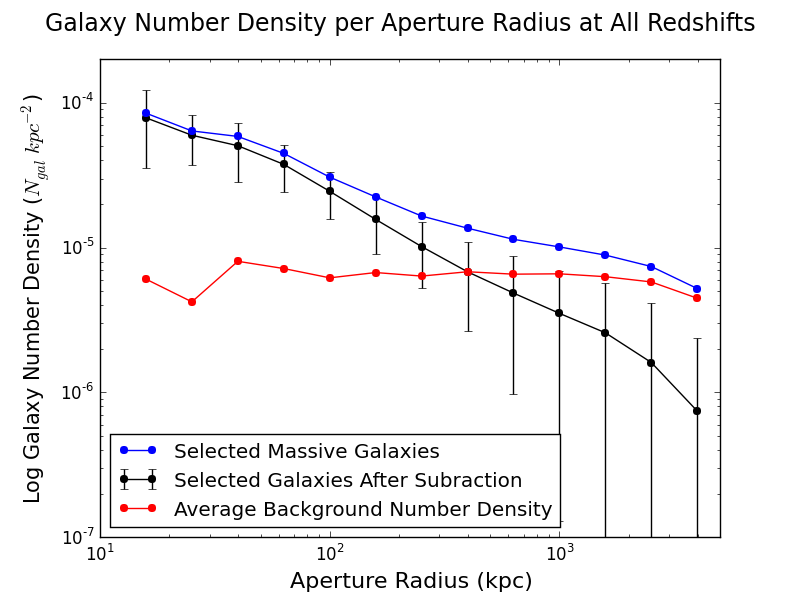
\includegraphics[width=\linewidth]{temp_compare}
\DeclareGraphicsExtensions{.png}
\caption{\footnotesize All galaxies plotted with number density compared to selected aperture radius. The average background number density per aperture radius is also included in red. The black line represents the average background number density subtracted from the calculated number density for all galaxies. The error bars show one standard deviation of thenumber density of the randomly selected background points at each aperture radius (the data used for the red line).}
\label{fig:compare}
\end{figure}

\subsection{Error Estimates}

A great source of error is the variation within the random background calculations for the aperture radius method. Beyond averaging four separate calculations, we show error bars for one standard deviation of the distribution of random background calculations for each galaxy within each radius. At low aperture radii, only a handful of galaxies in our sample selection actually conatain other galaxies. As a result, the average points in this data for low aperture radii are less accurate due to being averages of only a handful of galaxies rather than a few hundred. The radii affected by this are really only the lowest three. These two sources representsthe statistical uncertainty of our calculations.

There are various systematic unccertainties that could affect our data as well. Innacuracy in redshift and mass measurements could move galaxies in and out of both the general selected sample as well as specific bins within the sample. At extremely small aperture radii, source blending could cause a smaller than expected number density. 

\section{Results}

We primarily look at the evolution of local galaxy number density with respect to change in redshift, as Tal (2013)~\cite{2013ApJ...769...31T} did, but also with respect to mass. The main method we use is is counts in aperture radius, to allow analysis of both local and general environment, but the nth nearest method was also used to provide a more accurate study of the local environment.

\subsection{Redshift Evolution}

In studying the variation in galaxy number density with respect to redshift, we split the selected massive galaxies into four bins based on redshift: 0.5 \textless Z \textless 1.0, 1.0 \textless Z \textless 1.5, 1.5 \textless Z \textless 2.0, and 2.0 \textless Z \textless 2.5. We plot these four bins on a counts in aperture radius graph to show the variation in galaxy number density over different sized environments. The smaller aperture radii are less accurate due to a lack of statistical completeness. From the third aperture radius (about 40 kpc) on, one can assume sufficient statistical completeness due to most galaxies having at least a few others within that range. In a similar manner, the last two aperture radii (about 2.5 and 4 mpc) are slightly statistically incomplete due to many galaxies containing most of their entire field within that range. We see in figure~\ref{fig:z} that there is a clear trend for the majority of the plot. Lower redshifts correspond with higher galaxy number density, and high redshifts with low densities. 

\begin{figure}
\figurenum{2}
\centering
\graphicspath{{C:/3d_hst/2015_finals/aperture_distance/}}
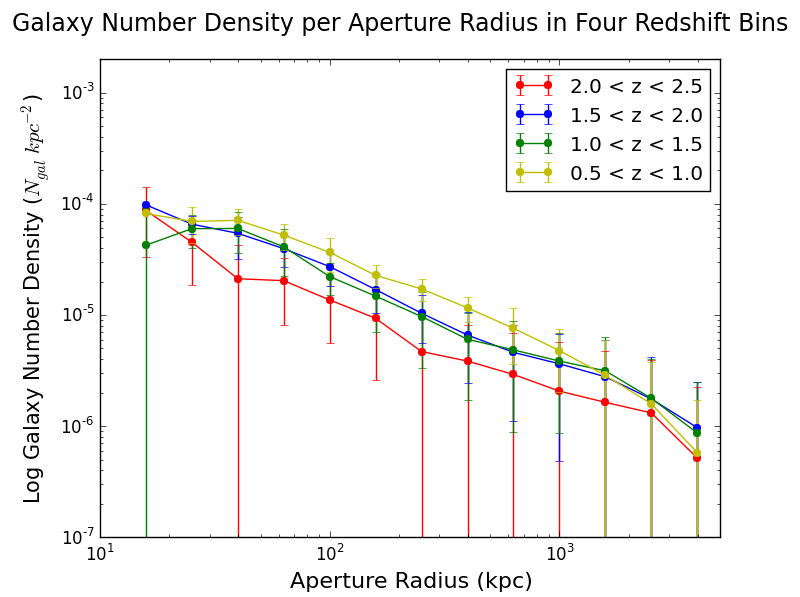
\includegraphics[width=\linewidth]{temp_z_final}
\DeclareGraphicsExtensions{.png}
\caption{\footnotesize All galaxies plotted in four redshift bins from 0.5 to 2.5. Galaxy number density is plotted with respect to aperture radius selected, both on logarithmic scales.  The lower redshifts have an increased galaxy number density in the aperture radius range of about 30 kpc to 1 mpc. Both extremes of the aperture radii can be largely ignored due to statistical incompleteness.}
\label{fig:z}
\end{figure}

We also compare this data with lower redshifts of the same plot from Tal (2013)~\cite{2013ApJ...769...31T} in figure~\ref{fig:zpanel}. Here we can see that his data shows a lower galaxy number density throughou, which can be attributed to the fact that he is using a different survey. Although the data seems very similar, Tal finds no evolution in galaxy number density with change in redshift, an interesting contrast with our data. 

\begin{figure}
\figurenum{3}
\centering
\graphicspath{{C:/3d_hst/2015_finals/aperture_distance/}}
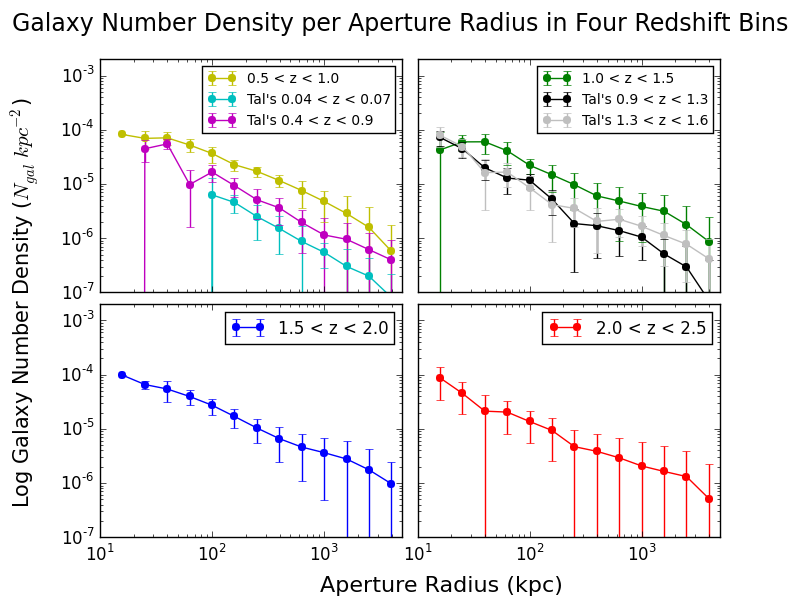
\includegraphics[width=\linewidth]{temp_zpanel_final}
\DeclareGraphicsExtensions{.png}
\caption{\footnotesize ZPANEL TEXT}
\label{fig:zpanel}
\end{figure}

\subsection{Variation over Mass}

In studying variation over mass, we once again split the selected massive galaxies into four mass bins: 10 \textsuperscript{11.0}$M_{\odot}$ \textless mass \textless 10 \textsuperscript{11.15}$M_{\odot}$, 10 \textsuperscript{11.15}$M_{\odot}$ \textless mass \textless 10 \textsuperscript{11.3}$M_{\odot}$, 10 \textsuperscript{11.3}$M_{\odot}$ \textless mass \textless 10 \textsuperscript{11.45}$M_{\odot}$, and mass \textgreater 10 \textsuperscript{11.45}$M_{\odot}$. The vast majority of the galaxies in the most massive bins lie between 10 \textsuperscript{11.45}$M_{\odot}$ and 10 \textsuperscript{11.6}$M_{\odot}$, but it should be mentioned that some are more massive up to a maximum of about 10 \textsuperscript{11.8}$M_{\odot}$. Just as with redshift, we plot the data on a counts in aperture radius graph in figure~\ref{fig:mass}. The only real takeaway from this plot is that there is a significant increase in galaxy number density for the most massive galaxies in the low and medium aperture radii.

\begin{figure}
\figurenum{4}
\centering
\graphicspath{{C:/3d_hst/2015_finals/nth_nearest/}}
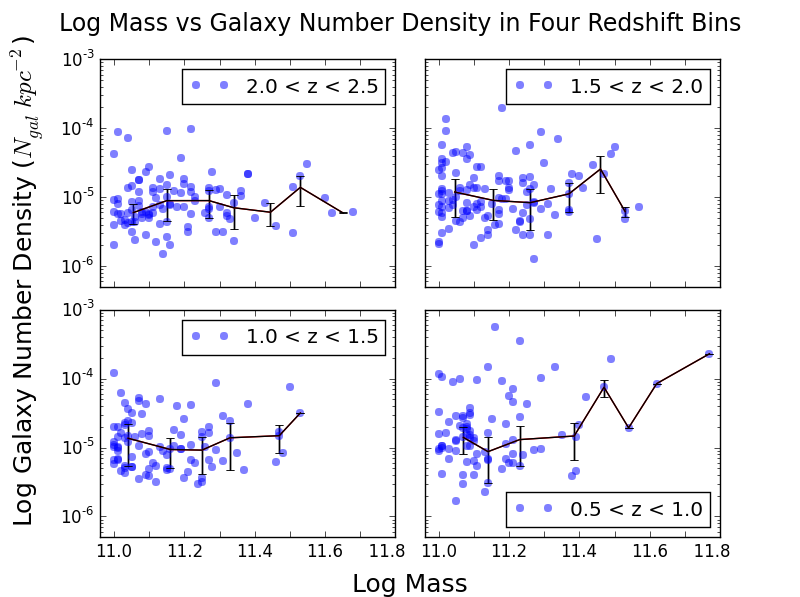
\includegraphics[width=\linewidth]{Mass_Density_Z}
\DeclareGraphicsExtensions{.png}
\caption{\footnotesize All of the galaxies sorted into four bins based on redshift and plotted with mass versus local galaxy number density (both on logarithmic scales). The black line represents the median point of eight mass bins for each subplot. There are error bars for the median absolute deviation of each median point. There is less variation of galaxy density with higher redshifts. An \textbf{\textit{n}} of 5 is used for the nth nearest calculation.}
\label{fig:nth}
\end{figure}

We also plot the data using the nth nearest method in figure~\ref{fig:nth}. In this plot we can analyze change in number density over both redshift and mass. The black line represents the median point for the galaxies, with error bars for the median absolute deviation. The trend of increased galaxy number density with lower redshifts is hard to see, but definively present. One can also notice a general upward trend of galaxy number density with increased mass, as seen in figure~\ref{fig:mass}. Beyond that, one can also see that there is less variation in galaxy number densities for all masses for higher redshifts (smaller error bars).

\begin{figure}
\figurenum{5}
\centering
\graphicspath{{C:/3d_hst/2015_finals/aperture_distance/}}
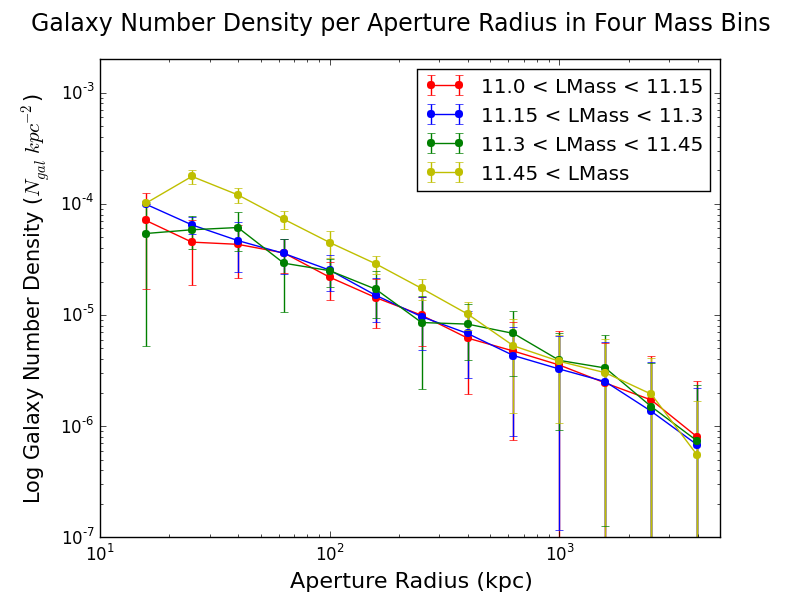
\includegraphics[width=\linewidth]{temp_lmass_final}
\DeclareGraphicsExtensions{.png}
\caption{\footnotesize All of the galaxies sorted into four bins based on mass. Galaxy number density is plotted against selected aperture radius. The error bars represent one standard deviation of the subtracted number density of the randomly selected background points. There is a significant increase in local galaxy number density for extremely high mass galaxies at distances less than 1 one megaparsec.}
\label{fig:mass}
\end{figure}

\section{Discussion}

What do these trends mean? I don't know


\acknowledgements

\appendix

\bibliographystyle{plain}
\bibliography{bibliography}

\end{document}
